\documentclass{article}

\begin{document}
\chapter{Implementation}

PLSI is designed to be portable to multiple technologies, CAD tool vendors, and
processor generators.  As such it has a modular system of addons that can be
mixed and matched in order to produce a chip.  Users are expected to define the
following variables, which will be used to control the flow:

\begin{itemize}
\item \texttt{CORE\_GENERATOR}
\item \texttt{SOC\_GENERATOR}
\item \texttt{TECHNOLOGY}
\item \texttt{SYNTHESIS\_TOOL}
\item \texttt{PAR\_TOOL}
\item \texttt{FORMAL\_TOOL}
\item \texttt{SIGNOFF\_POWER\_TOOL}
\item \texttt{SIMULATOR}
\end{itemize}

It is also possible to pass configuration information to each step in the flow
by setting the following variables

\begin{itemize}
\item \texttt{CORE\_CONFIG}
\item \texttt{CORE\_SIM\_CONFIG}
\item \texttt{SOC\_CONFIG}
\item \texttt{MAP\_CONFIG}
\end{itemize}

A top-level Makefile sequences the entire chip build; which includes running
all the CAD tools, testing the designs after every tool is run, and
interpreting the results.  A high-level overview of the PLSI flow can be seen
in Figure~\ref{impl:plsi-flow}.

\begin{figure}
\begin{center}
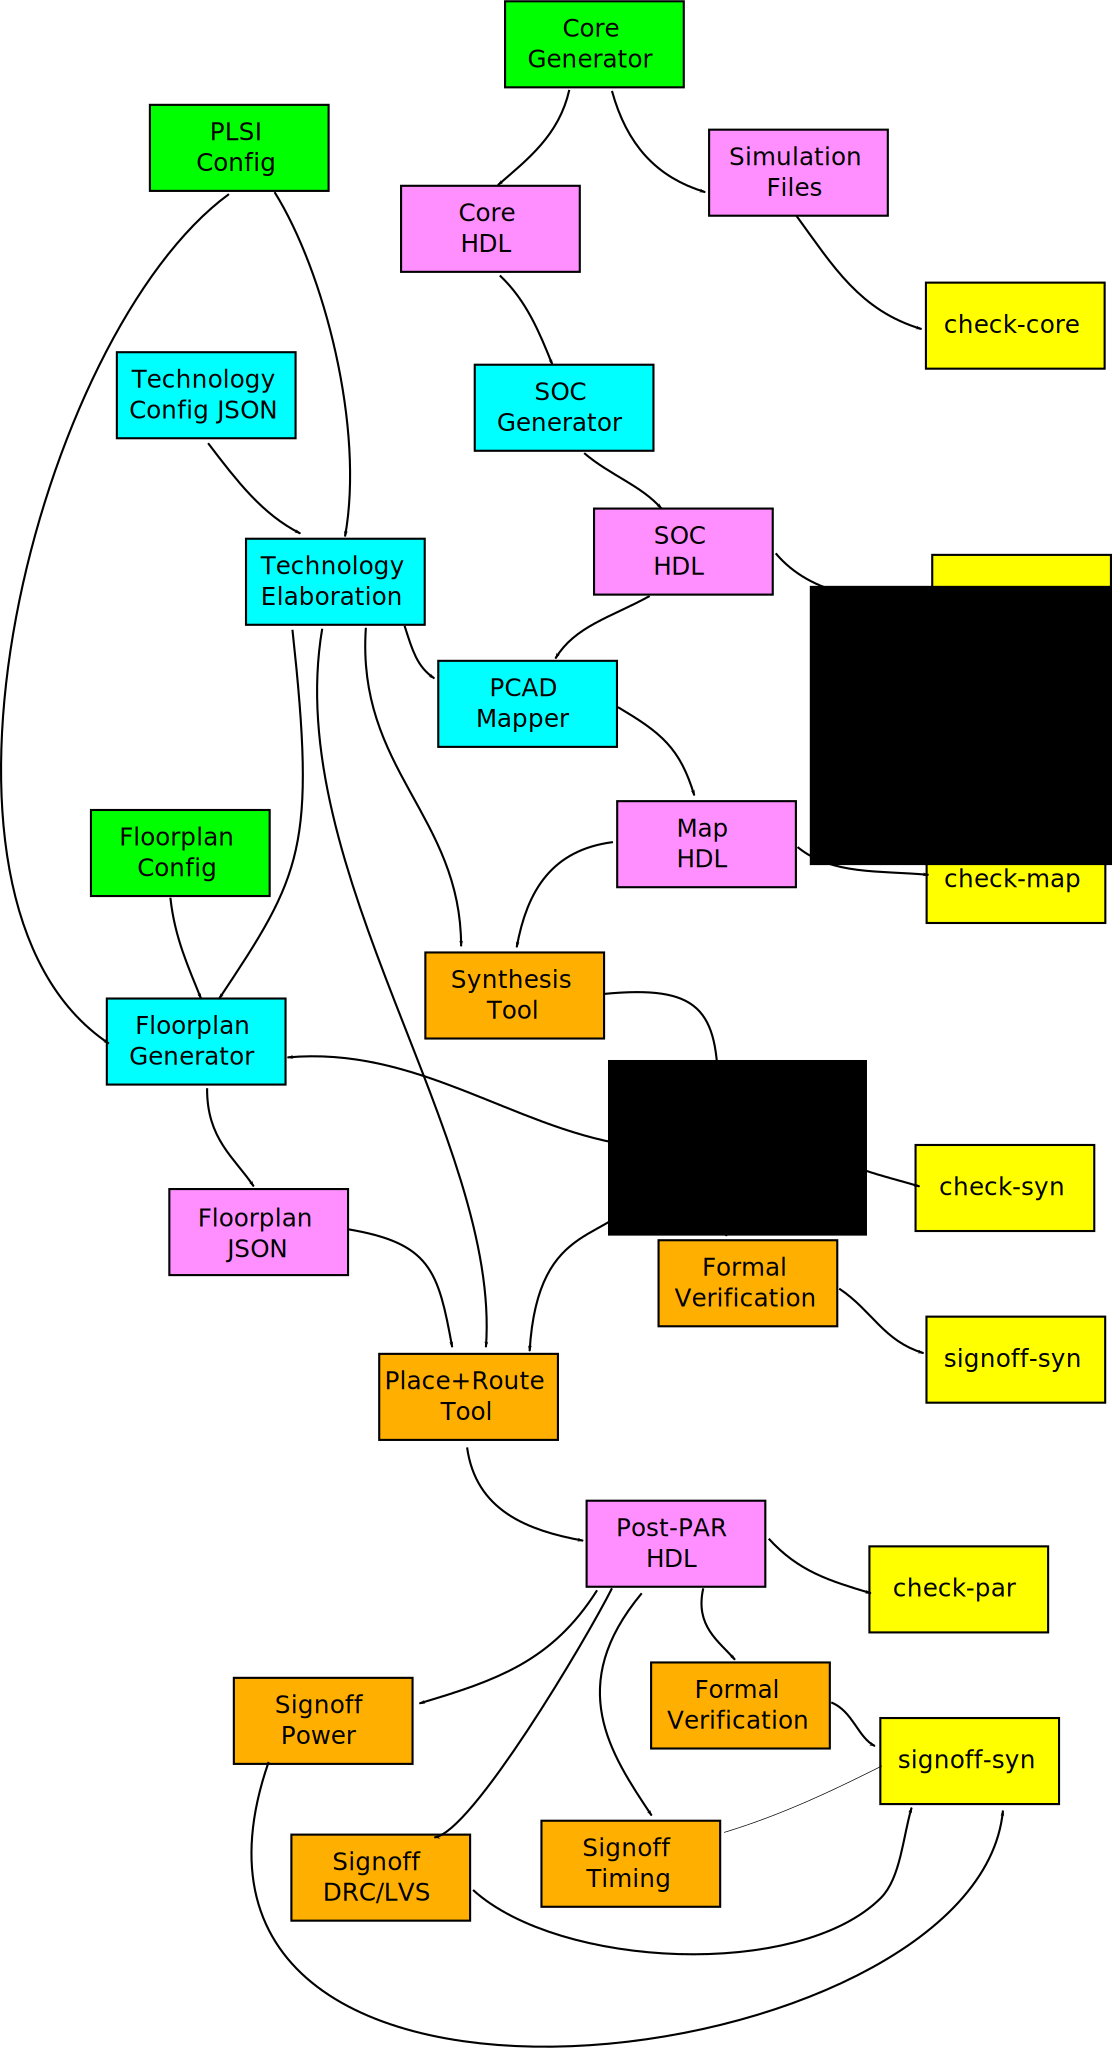
\includegraphics[width=0.7\linewidth]{figures/plsi-flow.svg}
\end{center}
\caption{A high-level overview of PLSI}
\label{impl:plsi-flow}
\end{figure}

\section{Core Generators}

PLSI was designed to support RTL-based research into microarchitectures by
quickly providing ground-truth power numbers for a large number of core
designs.  Thus the whole point of PLSI is that it is easy to port to new cores.
Porting PLSI to a new core generator based on Rocket Chip is extremely easy:
users simply need to point PLSI at their fork of Rocket Chip.  For example,
Figure~\ref{impl:hwacha-coregen} shows how little code is required to port PLSI
to the Hwacha vector unit.

\begin{figure}
\begin{verbatim}
CORE_DIR ?= $(CORE_GENERATOR_ADDON)/src/rocket-chip

RC_CORE_ADDONS = hwacha
CORE_TOP = ExampleTop

include src/addons/core-generator/rocketchip/vars.mk
\end{verbatim}
\caption{The core-generator addon for Hwacha}
\label{impl:hwacha-coregen}
\end{figure}

Porting PLSI to a core generator that isn't based on Rocket Chip is a bit more
involve.  The most interesting part of porting to PLSI is producing the list of
macros that the core requires.  There is a custom FIRRTL backend in PLSI that
allows Chisel based designs to easily generate PLSI macro configurations (this
tool is automatically used for Rocket Chip based projects), but Verilog based
cores have a bit more work to do.  I haven't actually managed to get a
reasonable open-source Verilog core, so I haven't ported PLSI to one yet.

\section{SOC Generators}

The SOC generation step converts a processor into an actual chip.  This means
inserting things like pads, clock recievers, etc.  For performing evaluations
of microarchitectures there is a ``nop'' SOC generator, which just doesn't do
anything.  This provides a simple way of evaluating a design without getting
into the complexities of chip building.  This was the only SOC generator used
for this thesis.

In addition to the ``nop'' SOC generator, there is also a ``bar-testchip'' SOC
generator.  This SOC generator generates a controller and phy that
transparently shims all top-level decoupled interfaces over a low-speed,
single-ended interface that is feasible to implement using the standard digital
IO pads that a popular commercial foundry provides.  This is designed to
provide a simple mechanism for building research-style test chips: it
alleviates the need to maintain chip-specific IO harnesses.  This SOC generator
was used to build a real chip on an agressive technology, but I've been removed
from the NDAs so I can't bring up the chip to see if it works or not.  The
process is completely automated: a PLSI tool reads to top-level Verilog of the
target design (using a Verilog parser I wrote), infers the decoupled
interfaces, generates an ASIC top-level wrapper and a test harness for both
FPGAs and simulation.

\section{Technology Mapping}

The technology mapping step converts generic macro implementations to those
that are specific to a particular technology.  This step is important to
maintaining portability of designs to multiple technologies: RTL writers should
never describe a technology-specific concept in their code but should instead
describe a generic version of that concept, which the mapping step then maps to
a technology-specific implementation.  This is really just a synthesis tool,
but it handles all the things that commercial synthesis tools don't understand.

The most important example of this is mapping sequential memories to SRAMs on
ASIC targets.  This is something that traditional synthesis tools can't do
because it's impossible to safely infer ASIC SRAMs from synthesizable Verilog.
Chisel and FIRRTL handle this mismatch by having an explicit memory visible to
the RTL programmer, which has been designed such that it can be mapped to ASIC
SRAMs.  PLSI uses this information to generate ASIC SRAM wrappers which can
then be passed on to the remainder of the CAD flow.

\subsection{Macro JSON Files}

PCAD has standardized on JSON as the interchange format between every step in
the flow because it's a well supported format.  The technology mapping step
expects a list of all the macros that need to be implemented and a list of all
the macros availiable to the technology.  Figure~\ref{impl:core-macro-list}
shows an example of one of the branch predictor memories in one of the BOOM
configurations, and Figure~\ref{impl:tech-macro-list} shows the ASIC SRAM that
will be used to implement that memory on the 32nm EDK.  

\begin{figure}
\begin{verbatim}
  {
    "type": "sram",
    "name": "h_table_ext",
    "depth": 32768,
    "width": 1,
    "ports": [
      {
        "clock port name": "RW0_clk",
        "mask granularity": 1,
        "output port name": "RW0_rdata",
        "input port name": "RW0_wdata",
        "address port name": "RW0_addr",
        "mask port name": "RW0_wmask",
        "chip enable port name": "RW0_en",
        "write enable port name": "RW0_wmode"
      }
    ]
  },
\end{verbatim}
  \caption{An example memory that needs to be mapped}
  \label{impl:core-macro-list}
\end{figure}

\begin{figure}
\begin{verbatim}
  {
    "family": "1rw",
    "width": 8,
    "name": "SRAM1RW1024x8",
    "ports": [
      {
        "write enable port name": "WEB",
        "clock port polarity": "positive edge",
        "output port polarity": "active high",
        "write enable port polarity": "active low",
        "address port polarity": "active high",
        "chip enable port polarity": "active low",
        "clock port name": "CE",
        "input port name": "I",
        "output port name": "O",
        "chip enable port name": "CSB",
        "read enable port name": "OEB",
        "input port polarity": "active high",
        "address port name": "A",
        "read enable port polarity": "active low"
      }
    ],
    "type": "sram",
    "depth": 1024
  },
\end{verbatim}
  \caption{An example ASIC SRAM macro description}
  \label{impl:tech-macro-list}
\end{figure}

\subsection{PCAD Macro Compiler}

In order to map technology-agnostic macros to technology-specific macros, I
implemented what is in effect a synthesis tool with a limited scope.  This tool
is an optimizing synthesis tool that uses some very simple optimization
techniques.  The only macro type I bother optimizing is the memories because
they're the only macros that I can compile that have any optimizations
potential.



\subsection{Technology JSON Files}

All the technology-specific information in PLSI is described within a single
file: the technology configuration file.  Defining all technology-specific
information in this manner is what allows PLSI backends to be portable to
multiple technologies.

An example technology JSON file is shown in Figure~\ref{impl:tech-json}.  As
you can see, technology JSON files describe where to download a technology
tarball from, how to extract that tarball, and the contents of that tarball.
It is possible to use scripts that operate on the post-extracted technology
PDKs to generate library fragments: for example, a script reads TSMC's memory
compiler documentation PDF to produce the list of SRAMs that compiler is
capable generating, which can then be passed to the PLSI macro compiler in
order to map arbitrary Chisel memories to TSMC SRAMs.

\begin{figure}
\begin{verbatim}
{
  "name": "An example technology",
  "tarballs": [
    "path": "tech.tar",
    "homepage": "http://example.com/technology",
  ],
  "libraries": [
    {
      "nldm liberty file": "tech.tar/lib/stdcell/tt0p9v25c.lib",
      "verilog file": "tech.tar/lib/stdcell.v",
      "corner": {
        "nmos": "typical",
        "pmos": "typical",
        "temperature": "25 C"
      },
      "supplies": {
        "VDD": "0.9 V",
        "GND": "0 V"
      }
    },
    {
      "nldm liberty file": "tech.tar/lib/sram1024x8/tt0p9v25c.lib",
      "provides": [
        "type": "sram",
        "width": 8,
        "depth": 1024,
        "ports": [
          {
            "read port name": "R",
            ...
          }
        ]
      ],
      ...
    }
  ]
}
\end{verbatim}
\caption{An example technology JSON file}
\label{impl:tech-json}
\end{figure}

When porting PLSI to a new technology it should only be necessary to create a
new technology JSON file (presumably patterned off a similar existing
technology JSON file).  In practice some modifications to all the tools that
consume the technology JSON files will be necessary, but the goal is that with
each new technology these modifications will become simpler and simpler.

\subsection{PLSI Configuration File}

PLSI must be provided with a configuration file in order to configure the
mapping phase.  This configuration file contains the additional information
needed to run the VLSI flow that is not present as part of the core generator.
An example PLSI configuration file is show in Figure~\ref{impl:plsi-config},
which is the default configuration file for mapping Rocket Chip's
\texttt{DefaultConfig} to the Synopsys 32nm educational PDK.  It's important to
note that while this config file is specific to a technology, it is independent
of the CAD tool vendors.

\begin{figure}
\begin{verbatim}
{
  "clocks": [
    {
      "name": "clock",
      "period": "1250ps",
      "par derating": "250ps"
    }
  ],
  "scenerios": [
    {
      "corner": {
        "nmos": "typical",
        "pmos": "typical",
        "temperature": "25 C"
      },
      "supplies": {
        "VDD": "1.05 V",
        "GND": "0 V"
      }
    }
  ]
}
\end{verbatim}
\caption{An example PLSI configuration file}
\label{impl:plsi-config}
\end{figure}

The PLSI configuration file is used to drive all the CAD tools that are run,
including both the proprietary ones via wrappers written for PLSI and tools
like the macro mapper that were written specifically for PLSI.  It allows users
to control chip-related settings that do not come from RTL, like the clock
speed and MCMM scenarios.

\section{Synthesis Tool Driver}

In order to be portable to multiple CAD tool vendors, PLSI expects that
pre-existing synthesis tools are wrapped up with a script that converts the
vendor-agnostic PLSI file formats into vendor-specific formats, runs the
synthesis tool, and verifies that the run completed without errors.  As a study
in portability, there are three synthesis tools supported: "yosys", an
open-source synthesis tool; "dc", Synopsys's Design Compiler; and "genus",
Cadence's GENUS synthesis tool.  Only basic features are supported for "yosys"
and "genus", while "dc" is the tool that was regularly used.

These wrapper scripts are pretty straight-forward.  In order to avoid copyright
violations, users are expected to have downloaded tarballs of the vendor's base
set of scripts.  PLSI then patches these scripts with patches that are
generated by reading the various synthesis inputs (the post-map verilog,
technology description file, and PLSI configuration file).  For example, in
order to produce a list of modules

\section{Floorplanning}

One of the more painful steps of producing ASIC results is floorplanning.  Our
floorplanning scripts have traditionally been non-portable even for similar
designs on the same process, much less across different processes.  In order to
allow floorplanning to be portable to multiple designs, tools, and processes
users write floorplan fragments in a Python DSL that was created for this
project.

PLSI's floorplanning system is based on generating hierarchical groups of
placeable elements, specifying hints as to how they should be arranged, and
nesting these groups.  The floorplanning DSL is designed to make it easy for
users to produce legal first-cut floorplans and then optimize them when trying
to actually build a chip.  This DSL handles the following pain points for users:

\begin{itemize}
\item Matching Chisel-generated names to logical floorplan groups.
\item Shaping logical floorplan groups.
\item Ordering macros within logical floorplan groups.
\end{itemize}

\subsection{SRAM Floorplanning}

The vast majority of the floorplanning work has gone into handling SRAM macros
for ASICs, since those are by far the most important QoR constraints when
building high performance processors.  The floorplanning step is
semi-automated: it's designed to make it easy for users to write first-cut
floorplans that apply to multiple design configurations while still allowing
them to fine-tine floorplans for maximum performance on the designs that end up
being interesting.

\begin{figure}
  \begin{verbatim}
class RocketTilePlacer:
  def __init__(self, config):
    self.top = None
    self.l1dd = []
    self.l1dm = []
    self.l1id = []
    self.l1im = []

  def insert(self, macro):
    if macro.matches(config.rtl_top):
      self.top = TopMacro(macro.name, macro.width, macro.height)
    elif macro.matches("coreplex/rocketTiles/dcache/data"):
      self.l1dd.append(macro)
    elif macro.matches("coreplex/rocketTiles/dcache/MetadataArray"):
      self.l1dm.append(macro)
    elif macro.matches("coreplex/rocketTiles/frontend/icache/u"):
      self.l1id.append(macro)
    elif macro.matches("coreplex/rocketTiles/frontend/icache/tag_array/tag_array"):
      self.l1im.append(macro)
    else:
      print("%s cannot be matched" % macro.name)
      return False
    return True

  def list_constraints(self):
    l1dd = TopLeftPlacer   (self.top, self.top.tl(), sorted(self.l1dd))
    l1dm = TopLeftPlacer   (self.top, l1dd.bl(),     sorted(self.l1dm), self.top.width * 0.75)
    l1id = BottomLeftPlacer(self.top, self.top.bl(), sorted(self.l1id))
    l1im = BottomLeftPlacer(self.top, l1id.tl(),     sorted(self.l1im), self.top.width * 0.75)
    return l1dd.place() + l1dm.place() + l1id.place() + l1im.place()
\end{verbatim}

  \caption{Example Rocket Floorplan}
  \label{impl:example-floorplan}
\end{figure}

Figure~\ref{impl:example-floorplan} shows the floorplanning script for a single
Rocket core without an L2.  As you can see, users can write any Python code
they want to control floorplans in as much detail as they want -- even
providing absolute coordinates for every floorplanable block if they so desire.
The canonical way to write floorplans in PLSI is to use the demonstrated
helpers to write floorplans in a more technology-agnostic way.

For example, the floorplan demonstrated in Figure~\ref{impl:example-floorplan}
should work on any of the technologies I have had access to, and should work
for any reasonable configuration of Rocket.  This floorplan puts the data RAMs
for the instruction and data caches on opposite sides of the chip and puts the
metadata RAMs in between, limiting the width of the metadata blocks to $75\%$
of the total chip width in order to avoid entirely blocking off the data RAMs
on pathological technologies (like SAED32) where Rocket's L1 metadata maps very
poorly to the available SRAMs.

\begin{figure}
  \begin{center}
    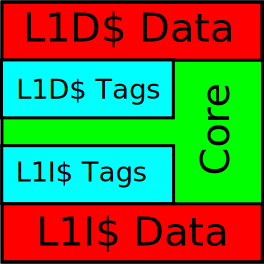
\includegraphics[width=0.95\linewidth]{figures/rocket-floorplan-general.svg}
  \end{center}
  \caption{Generalized version of the example floorplan from Figure~\ref{impl:example-floorplan}}
  \label{impl:example-floorplan-output}
\end{figure}

\begin{figure}
  \caption{Concrete version of the example floorplan from Figure~\ref{impl:example-floorplan}, on SAED32}
  \label{impl:example-floorplan-saed32}
\end{figure}

\subsection{Power Floorplanning}

Almost no work has gone into power floorplanning in PLSI: you just get a single
power domain with rings around the outside of the chip's routeable area and a
grid inside the rings on the highest metal layers available for regular
routing.  This power floorplan should be sufficient to evaluate
microarchitectures and to build simple chips, but isn't enough to build
a big chip.

\section{Place and Route Tool Driver}

Much like the synthesis tool driver, the place and route tool driver takes in
various vendor-agnostic file formats, converts them to vendor-specific formats
when necessary, runs the vendor's synthesis tool, checks to see that there are
no errors, and then produces the results for other steps to use.

The only PAR tool driver I bothered implementing was for ICC, since it is the
only one that works with the 32nm Synopsys educational PDK.

\end{document}
